\section{Teoria Dei Codici}
    \subsection{Introduzione}
        Ci concentriamo adesso sul trattamento dell'informazione per poterla trasmettere.
        I messaggi che trasmettiamo possono essere codificati per vari motivi:
        \begin{itemize}
            \item {
                    Compressione:$\begin{cases}
                        \text{Lossy: con perdita dell'informazione} \nonumber\\
                        \text{Lossless: minima perdita dell'informazione} \nonumber
                    \end{cases}$\\
                    Comprimere l'informazione in elimenando ridondanza e salvando spazio di memoria e banda.
                    
                }
            \item {
                    Crittografia: per nascondere il messaggio ad utenti in ascolto sul canale che non siano il destinatario.
            }
            \item {
                    Rivelazione o correzione di errore: vieen aggiunta ridondanza ad hoc per aumentare l'affidabilitá del messaggio trasmesso. 
                    Si utilizzano \href{https://en.wikipedia.org/wiki/Checksum}{checksum} o \href{https://en.wikipedia.org/wiki/Reed-Solomon_error_correction}{Reed-Solomon(RS)}
            }
        \end{itemize}
        \paragraph{Capacitá del canale}\label{Capacita del canale}\index{Capacitá del canale}
            La capacitá del canale $C$ indica la massima quantitá d'informazione che puó essere trasmessain maniera affidabile su di un dato canale.
            La capacitá dipende dalla banda $B$ del canale e dal rapporto segnale rumore (signal-to-noise ratio,\href{https://en.wikipedia.org/wiki/Signal-to-noise_ratio}{$SNR$}):
            \[
                C = B\log(1 + SNR)  
            \] 
        \paragraph{Canale Gaussiano}\index{Canale Gaussiano}
            Il canale Gaussiano puó essere modellato come \href{https://en.wikipedia.org/wiki/Binary_symmetric_channel}{Binary Symmetric Channel (BSC)} con probabilitá di errore $p$. 
            Assumiamo gli errori tra loro indipendenti ($p_{(a,b)} = p_{(a)}\dotproduct p_{(b)}$):
        \begin{figure}[H]
            \centering
            \includegraphics[width = 12cm]{media/600px-Binary_symmetric_channel_(en).svg.png}
            \label{BSC system}
            \caption{Sistema di trasmissione BSC}
        \end{figure}
        \begin{gather}
            E_{(x)}: \text{Funzione di codifica} \nonumber \\
            D_{(x)}: \text{Funzione di decodifica} \nonumber \\
            E_{(m)}: \text{Bit dell'informazione codificati} \nonumber \\
            y^\prime: E_{(m)}+ e \rightarrow \text{Informazioni con errore del canale} \nonumber \\
            m = D_{(y^\prime)}: \text{Informazione decodificata} \nonumber 
        \end{gather}
        Il canale é chiamato simmetrico perché ho la stessa probabilitá errore sulla trasmissione di uno dei due bit.
        Se $X$ é il bit inviato e Y quello ricevuto allora il canale é caratterizzato dalle probabilitá:
        \begin{align}
            P(Y=0|X=0) &= 1-p\nonumber \\
            P(Y=0|X=1) &= p\nonumber \\
            P(Y=1|X=0) &= p\nonumber \\
            P(Y=1|X=1) &= 1-p\nonumber 
        \end{align} 
        Assumiamo che $0\leq p \leq\frac{1}{2}$, se avessimo $p >\frac{1}{2}$ il ricevitore potrebbe scambiare l'informazione ricevuta
        (Quando riceve un $1$ lo interpreta come $0$ e viceversa) e ottenere un canale con probabilitá $1-p \leq\frac{1}{2}$. 
        
        Nel corso useremo delle simbologie diverse:
        \begin{figure}[H]
            \centering
            \includegraphics[width = 12cm]{media/BSC System.png}
            \label{BSC system moretti}
            \caption{Sistema di trasmissione BSC}
        \end{figure}
        \begin{gather}
            u: \text{Informazione} \nonumber \\
            x: \text{Parole di Codice} \nonumber \\
            e: \text{Errore del Canale} \nonumber \\
            y: x+e \rightarrow \text{Informazioni con errore del canale} \nonumber \\
            \overset{\wedge}{x}: \text{Informazione decodificata} \nonumber 
        \end{gather}
        \paragraph{Probabilitá di errore BSC}\label{Probabilita di errore BSC}\index{Probabilitá di errore BSC}
            La probabilitá, per una trasmissione BSC, di sbagliare $t$ bit in una parola di $n$ bit:
            \[
                p_{(t,n)} = \binom{n}{t} p^t (1-p)^{(n-t)}
            \]
            dove il coefficente binomiale:
            \[
                \binom{n}{t} = \frac{n!}{t!(n-t)!}
            \]
            indica tutte le possibili combinazioni di errori di $t$ bit su $n$ bit. 
        \paragraph{Tassonomia dei codici}
            \begin{itemize}
                \item {Codici lineari
                        \begin{itemize}
                            \item {
                                Codici a blocco
                                }
                            \item{
                                Codici convoluzionali
                            } 
                        \end{itemize}
                    }
                \item {
                    Definizione di un codice a blocco: 
                    \begin{figure}[H]
                        \centering 
                        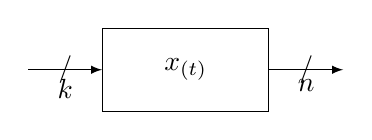
\begin{tikzpicture}[
                            node distance=2cm,
                            >=latex
                            ]

                            \node [coordinate] (input) {};
                            \node [draw, rectangle,right of = input, minimum height=3em, minimum width=6em] (block) {$x_{(t)}$};
                            \node [coordinate, right of = block] (output) {};
                            
                            \draw[draw,->] (input) -- node[midway]{$/$} node[below]{$k$} (block);
                            \draw[->] (block) -- node[midway]{$/$} node[below]{$n$} (output);
                        \end{tikzpicture}    
                    \label{Def codice a blocco}
                    \end{figure}
                    \paragraph{Rate del Codice}:\index{Rate del Codice}
                        {
                            \[
                                R = \frac{k}{n}  
                            \]
                            La condizione é che $n>k$ senon fosse cosí avrei perdita d'informazione, da $k$ bit passo a $n$ aggiungendo
                            ridondanza e codificando i miei dati. Possiamo quindi stimare il valore tipico di $R$
                            \[
                                R = \frac{k}{n} <1  
                            \]
                        }
                }
                \item Rivelazione di errore:\index{Rivelazione di errore}{
                    Consiste nella capacità di scoprire la presenza di errori causati dal rumore o da altri fenomeni deterioranti 
                    durante una trasmissione di dati (es. tramite il \href{https://it.wikipedia.org/wiki/Bit_di_parit%C3%A0}{bit di paritá}).
                }
                \item {Correzione di errore:\index{Correzione di errore}{
                    Consiste invece nell'ulteriore abilità di ricostruire i dati originali, eliminando gli errori occorsi durante la trasmissione.
                    Vi sono due differenti schemi di base per la progettazione della codifica di canale e del protocollo per un sistema che corregge gli errori:
                    \begin{itemize}
                        \item {
                            ??\href{https://it.wikipedia.org/wiki/Automatic_repeat-request}{Automatic repeat-request} (ARQ): Il mittente invia i dati ed anche un codice a rilevazione d'errore, che sarà
                            utilizzato in ricezione per individuare gli eventuali errori, ed in tal caso chiedere la ritrasmissione dei dati
                            corrotti. In molti casi la richiesta è implicita; il destinatario invia un acknowledgement (ACK) di corretta 
                            ricezione dei dati, ed il mittente re-invia solo quei dati per i quali non ha ricevuto, entro un prefissato tempo 
                            limite (timeout), il corrispondente ACK.
                        }
                        \item{
                            ??\href{https://it.wikipedia.org/wiki/Forward_Error_Correction}{Forward Error Correction} (FEC): Il mittente codifica i dati con un codice a correzione d'errore 
                            (error correction code, ECC) ed invia il messaggio codificato. Il destinatario non invia mai alcun 
                            messaggio verso il mittente; esso decodifica ciò che riceve nella maniera più simile possibile a quella di un 
                            certo insieme prefissato di parole accettabili. Tali codici sono realizzati in modo tale che dovrebbe occorrere 
                            una quantità "irragionevole" di errori nei dati, affinché il destinatario decodifichi erroneamente, ottenendo 
                            finalmente dei dati diversi da quelli effettivamente inviatigli.
                        } 
                    \end{itemize}
                    In generale un codice a blocco che ha rate $\frac{k}{n}$ mappa $k$ bit su $n$ bit usando $2^k$ parole di codice di dimensione n
                }}
            \end{itemize}

        \subsubsection{Esempio codici a blocco: codici a ripetizione}
            É un esempio di codice a correzione d'errore: il funzionamento si basa sulal ripetizione dell'informazione piú volte. Il destinatario
            si accorge di un errore di trasmissione poiché il flusso di dati ricevuto non è la ripetizione di un singolo messaggio e, inoltre, 
            il destinatario può recuperare il messaggio originale guardando il messaggio ricevuto nel flusso di dati che si verifica più spesso.

            Nel caso di un codice binario di ripetizione, esistono due parole in codice - tutte uno e tutti zeri - che hanno una lunghezza n. 
            Pertanto, la distanza minima di Hamming (\ref{Distanza di Hamming}) del codice è uguale alla sua lunghezza. Ciò conferisce al codice 
            di ripetizione, con $R = \frac{1}{n}$,una capacità di rivelazione di errori pari a $n-1$ e correzione degli errori (cioè correggerà fino agli errori in qualsiasi parola del codice) di $\frac{n-1}{2}$ per n dispari(\ref{Probabilita di errore BSC}).\\
            Esempio:\\
            \indent{$R = \frac{1}{3} \rightarrow$ ha solo 2 parole di codice:}
            \begin{align}
                u=0 \rightarrow x = [000]\nonumber \\
                u=1 \rightarrow x = [111]\nonumber
            \end{align} 
            Il ricevitore effettua una decodifica a maggioranza: decide per il bit che comprare piú volte della parola ricevuta.
            \begin{align}
                y = [000] \rightarrow \overset{\wedge}{x} = [000] \rightarrow \overset{\wedge}{u} = 0 \nonumber \\
                y = [010] \rightarrow \overset{\wedge}{x} = [000] \rightarrow \overset{\wedge}{u} = 0 \nonumber \\
                y = [101] \rightarrow \overset{\wedge}{x} = [111] \rightarrow \overset{\wedge}{u} = 1 \nonumber
            \end{align}
            \paragraph{Evento errore:} l'evento errore per un codice a correzione di errore consiste nel non essere in grado di correggere
            tutti gli errori introdotti dal canale. Se la probabilitá di errore sul bit $p_{e,b}$ é piccola, la probabilitá di errore 
            $p_{e,W}$ per il codice puó essere approssimata dal primo evento che determina la ricezione errata (nel caso dei codici a ripetizione a $R = \frac{1}{3}$ 
            si verifichino $2$ errori).
            \begin{itemize}
                \item {$R = \frac{1}{3}$
                    \begin{itemize}
                        \item {
                            Se $p_{e,b} = 0.1 \Rightarrow p_{e,W} \approx 2.7\dotproduct 10^{-2} $ 
                        }
                        \item {
                            Se $p_{e,b} = 0.01 \Rightarrow p_{e,W} \approx 2.97\dotproduct 10^{-4} $ 
                        }
                    \end{itemize}
                }
                \item {$R = \frac{1}{5}$
                    \begin{itemize}
                        \item {
                            Se $p_{e,b} = 0.1 \Rightarrow p_{e,W} \approx 8.1\dotproduct 10^{-3} $ 
                        }
                        \item {
                            Se $p_{e,b} = 0.01 \Rightarrow p_{e,W} \approx 9.8\dotproduct 10^{-6} $, Sviluppiamo i calcoli come esempio: 
                            \[
                                P_r \{\text{codice }R=\frac{1}{5}\text{ non riesce a correggere gli errori introdotti dal canale}\}:
                            \]
                            \begin{align}
                                P_r &= \sum_{t=3}^{5} \binom{5}{t}p^t (1-p)^{5-t},\hspace{0.2cm} p=10^{-2} \nonumber \\
                                P_r &\{\text{3 errori su 5}\}= \binom{5}{3}p^3 (1-p)^{5-3} = 10\dotproduct 10^{-6} (0.99)^2 = 9.8\dotproduct 10^{-6} \nonumber \\
                                P_r &\{\text{3 errori su 5}\}= \binom{5}{4}p^4 (1-p)^{5-4} = 5\dotproduct 10^{-8} (0.99) = 5\dotproduct 10^{-8}\nonumber \\
                                P_r &\{\text{3 errori su 5}\}= \binom{5}{5}p^5 (1-p)^{5-5} = 1\dotproduct 10^{-10} = 10^{-10}\nonumber 
                            \end{align}
                        }
                    \end{itemize}
                }
            \end{itemize}

        \subsubsection{Esempio codici a blocco: codici a controllo di paritá}
        Il bit di parità è un codice di controllo d'errore, utilizzato nei calcolatori per prevenire errori nella trasmissione o nella memorizzazione dei dati. 
        Tale codice prevede l'aggiunta di un bit ridondante ai dati, calcolato a seconda che il numero di bit che valgono 1 sia pari o dispari. Ne esistono
        quindi 2 varitá: bit di paritá pari e bit di paritá dispari. Quando si usa il bit di paritá pari si aggiunge un bit con valore $1$ se nella parola inviata
        il numero di occorrenze di "$1$" é dispari(portando il numero di occorrenze di "$1$" a una quantitá pari).Quando si usa il bit di paritá dispari si
        aggiunge un bit con valore $1$ se nella parola inviata il numero di occorrenze di "$1$" é pari (portando il numero di occorrenze di "$1$" a una quantitá dispari).

        \noindent Il codice ha $R = \frac{k}{(k+1)}$: $k$ bit informativi piú il bit di paritá.
        
        \paragraph{Rilevazione dell'errore:}La rilevazione d'errore deriva dalla discordanza del numero di occorrenze di "$1$", eseguendo lo XOR bit a bit, nel caso del bit di paritá pari, se il risultato
        é $0$ non sono avvenuti errori, viceversa se ho un risultato uguale a $1$ posso dire che cé stato uno o una quantitá dispari di errori nella trasmissione, questo lo rende
        solo un codice a rilevazione d'errore e non un codice a correzione d'errore.
        
        Esempio:Trasmetto parole di $11bit$ con rate $R_b = 10Mb/s$ e probabilitá di errore sul bit trasmesso $p_{e,b} = 10^{-8}$:
        \begin{itemize}
            \item {
                Senza controllo di paritá é sufficiente che sia sbagliato anche un solo bit per sbagliare tutta la parola:
                \[
                    p_{e,W} = \sum_{j=1}^{11} \binom{11}{j}p_{e,b}^j (1-p_{e,b})^{11-j} = 11 p_{e,b} (1-p_{e,b})^{10} \simeq 11p_{e,b}
                \]
                ed il rate di parole sbagliate al secondo é:
                \[
                    R_{e,W} = \frac{R_b}{11}\dotproduct p_{e,W} \simeq \frac{10^7}{11}\dotproduct 11p_{e,b} = 0.1_\frac{w}{s}
                \]
            }
            \item {
                Aggiungendo un bit di paritá, la parola diventa di 12 bit e sbaglio quando faccio almeno 2 errori, il singolo errore
                viene corretto chiedendo nuovamente la trasmissione del dato:
                \[
                    p_{e,W} = \sum_{j=2}^{12} \binom{12}{j}p_{e,b}^j (1-p_{e,b})^{12-j} = 66 p_{e,b}^2 (1-p_{e,b})^{10} \simeq 66p_{e,b}^2
                \]
                ed il rate (frequenza) di parole sbagliate al secondo é:
                \[
                    R_{e,W} = \frac{R_b}{12}\dotproduct p_{e,W} \simeq \frac{10^7}{12}\dotproduct 66p_{e,b}^2 = 5.5\dotproduct 10^{-9} \frac{w}{s}
                \]
                possiamo anche calcolare il periodo $T_{e,W} = \frac{1}{R_{e,W}} =  1.82\dotproduct 10^{8} s$ che é una parola ogni sei anni circa.  
            }
        \end{itemize}
        \subsubsection{Esempio codici a blocco: codice ISBN}
            Il codice International Standard Book Number (ISBN) é un codice a controllo di paritá per un alfabeto di simboli nonbinari. 
            Ad ogni libro é assegnata una parola di codice di lunghezza $n=10$ cifre in base decimale. Le prime 9 cifre identificano il libro, 
            la decima é quella di controllo di paritá cosí calcolata:
            \begin{enumerate}
                \item {
                    Si calcola la grandezza $z = mod(S,11)$ con
                    \[
                        S = \sum_{j=1}^{9} (11-j)x_{(j)}
                    \]
                }
                \item {
                    La cifra di controllo di aritá é il complemento a 11 di $z$:
                    \[
                        x_{(10)} = mod(11-z,11)  
                    \]
                    E solo per la cifra di controllo di paritá se $x_{(10)} = 10$ si sostituisce con 
                    $x_{(10)} = X$
                }
            \end{enumerate}
            Quando un dispositivo legge il codice lo verifica come segue:
            \begin{enumerate}
                \item {
                    Moltiplica ogni cifra per il peso della posizione della stessa cifra e calcola $mod(S^\prime,11)$ con
                    \[
                        S^\prime = \sum_{j=1}^{10} (11-j)y_{(j)}
                    \]
                }
                \item {
                    Assumendo che non ci siano errori su $x_{(10)} = |11-z|_{11}$, si ha:
                    \begin{align}
                        mod(S^\prime,11) &= mod \left( \sum_{j=1}^{9} (11-j)y_{(j)} + mod(11-z,11),11\right) \nonumber \\
                                         &= mod \left( \sum_{j=1}^{9} (11-j)y_{(j)} + \left(11-\sum_{j=1}^{9} (11-j)x_{(j)}\right),11\right)\nonumber \\
                                         &= mod \left(\sum_{j=1}^{9} (11-j)(y_{(j)}-x_{(j)}),11\right)
                    \end{align}
                }
            \end{enumerate}
            Se non ci sono errori si ha $y=x$ e quindi il $mod(S^\prime,11) = 0$
            \paragraph{Rivalazione degli errori:} Il codice é in grado di rivelare tutti i singoli errori:
            sia $e_{(k)}$ l'errore in posizione $k$,$y_{(k)} = x_{(k)}+ e_{(k)}$:
            \[
                mod(S^\prime,11) = mod((y_{(k)}-x_{(k)})(11-k),11)+mod(e_{(k)}(11-k),11) \neq 0
            \]
            Il codice é in grado di rivelare tutti i casi in cui ci sia uno scambio di 2 cifre del codice. Siano 
            $k_1$ e $k_2$ le 2 posizioni scambiate:
            \begin{align}
                mod(S^\prime,11) &= mod \left((y_{(k_1)}-x_{(k_1)})(11-k_1)+(y_{(k_2)}-x_{(k_2)})(11-k_2),11\right) \nonumber \\
                                 &= mod \left((x_{(k_2)}-x_{(k_1)})(11-k_1)+(x_{(k_1)}-x_{(k_2)})(11-k_2),11\right)\nonumber \\
                                 &= mod \left((x_{(k_2)}-x_{(k_1)})(k_2-k_1),11\right) \neq 0 \nonumber
            \end{align}
            Esempi:
            \begin{itemize}
                \item {Senza errore:
                    \begin{align}
                        ISBN & = 01-333-5485-7 \nonumber \\
                        \left| S^\prime \right|_{11} &= 0\dotproduct 10 +1\dotproduct 9+3\dotproduct 8+3\dotproduct 7+3\dotproduct 6+5\dotproduct 5+4\dotproduct 4+8\dotproduct 3+5\dotproduct 2+7\dotproduct 1\nonumber \\
                        \left| S^\prime \right|_{11} &= \left| 154 \right|_{11} = 0 \nonumber 
                    \end{align}
                    Il codice é corretto 
                }
                \item {Con errore: Scambio le cifre
                    \begin{align}
                        ISBN & = 01-333-5458-7 \nonumber \\
                        \left| S^\prime \right|_{11} &= 0\dotproduct 10 +1\dotproduct 9+3\dotproduct 8+3\dotproduct 7+3\dotproduct 6+5\dotproduct 5+4\dotproduct 4+{\color{red}5\dotproduct 3}+{\color{red}8\dotproduct 2}+7\dotproduct 1\nonumber \\
                        \left| S^\prime \right|_{11} &= \left| 151 \right|_{11} = 8 \neq 0 \nonumber 
                    \end{align}
                    Il codice non é corretto 
                }
            \end{itemize}
        \subsection{Codici a blocco}
        \subsubsection{Introduzione ai codici lineari}
            \paragraph{Campo:} un campo é una struttura composta da un insieme non vuoto $F$ e da due operazioni binarie interne: $\forall \alpha,\beta,\gamma \in F$:
                \begin{itemize}
                    \item {
                        Somma ($XOR$):
                        \begin{itemize}
                            \item {
                                \[
                                    \alpha + \beta = \theta, \theta \in F  
                                \]
                            }
                            \item {Associativa:
                                \[
                                    (\alpha + \beta) + \gamma = \alpha +( \beta + \gamma)
                                \]
                            }
                            \item {Commutativa:
                                \[
                                    \alpha + \beta = \beta + \alpha
                                \]
                            }
                            \item {Elemento Neutro:
                                \[
                                    0\in F,\alpha + 0 = \alpha,\alpha-\alpha = 0
                                \]
                            }
                        \end{itemize}
                    }
                    \item {
                        Prodotto ($AND$):   
                        \begin{itemize}
                            \item {
                                \[
                                    \alpha \dotproduct \beta = \theta, \theta \in F  
                                \]
                            }
                            \item {Associativa:
                                \[
                                    (\alpha \dotproduct \beta) \dotproduct \gamma = \alpha \dotproduct( \beta \dotproduct \gamma)
                                \]
                            }
                            \item {Commutativa:
                                \[
                                    \alpha \dotproduct \beta = \beta \dotproduct \alpha
                                \]
                            }
                            \item {Distributiva:
                                \[
                                    (\alpha + \beta) \dotproduct \gamma = \alpha \dotproduct \gamma + \beta \dotproduct \gamma
                                \]
                            }
                            \item {Elemento Neutro:
                                \[
                                    1\in F,\alpha \dotproduct 1 = \alpha,\forall \alpha \neq 0\rightarrow \alpha\dotproduct\alpha^{-1} = 0
                                \]
                            }
                        \end{itemize}
                    }
                \end{itemize}
        \subsubsection{Campi di Galois}
            Un campo finito, detto anche campo di Galois, é un campo con un numero finito $q$ di elementi. Il numero di elementi di definisce la categoria del
            campo: $GF(2)$ é il campo definito su $\{0,1\}$ con somma modulo 2 ($XOR$) e prodotto modulo 2 ($AND$). Definito lo spazio $GF(2)$ si puó costruire
             lo spazio vettoriale $\mathcal{V}_n=GF(2)^2$, lo spazio di tutti i possibili $2^n$ vettori di $n$ cifre binarie su cui valgono le operazioni definite per 
             $GF(2)$.

        \subsubsection{Codici a blocco lineari su $GF(2)$}
            Sia $u = [u_1, \dots, u_k]$ una generica parola di $k$ cifre binarie. Il codice a blocco lineare $\mathcal{C}(k,n)\subset \mathcal{V}_n$ é l'insieme delle
            $2^k$ parole $x = [x_1, \dots, x_n]$ di $n$ cifre binarie ottenute con la trasformazione lineare:
            \[
                x = uG  
            \]
            Dove $G$ é la matrice generatrice del codice e ha dimensione $k \times n$ di cifre binarie con $n>k$ poiché al massimo
            aggiungo informazioni per la trasmissione, per la correzione o rivelazione d'errore.
            
            Siano $g_i, i = [1, \dots, k]$, le righe di $G$, $x$ é la combinazione lineare delle righe $g_i$:
            \[
                x = \sum_{i=1}^{k}u_ig_i  
            \]
            Per avere $2^k$ parole di codice distinte  é necessario che $G$ abbia rango $k$: le righe di $G$ devono essere linearmente indipendenti e costituiscono 
            una $base$ per il sottospazio vettoriale $\mathcal{C} \subset \mathcal{V}_n$.  

        \subsubsection{Propietá dei codici a blocco lineari}
            Le propietá derivano maggiormente dalla pripietá di linearit;a dei codici:
            \begin{itemize}
                \item {Ogni parola di codice é una combinazione lineare di righe della matrice generatrice.}
                \item {Il codice a blocchi é costituito da tutte le possibili combinazioni delle righe della matrice generatrice.}
                \item {La somma di due parle di codice é ancora una parola di codice.}
                \item {La $n-upla$ di tutti zeri é sempre una parola di codice.}
                \item {Se $x$ é una parola di codice, anche $-x$ é una parol di codice.}
            \end{itemize}

        \subsubsection{Distanza di Hamming}\label{Distanza di Hamming}\index{Distanza di Hamming}
            La distanza di Hamming tra due vettori, o stringhe, $d(x_1,x_2)$ di $n$ elementi é il nuemro di posizioni in cui le due parole
            sono diverse tra loro. Esempi:
            \begin{itemize}
                \item {
                    La distanza di Hamming tra 10{\color{red}1}1{\color{red}1}01 e 10{\color{red}0}1{\color{red}0}01 è 2.
                }
                \item {
                    La distanza di Hamming tra 2{\color{red}14}3{\color{red}8}96 e 2{\color{red}23}3{\color{red}7}96 è 3.
                }
            \end{itemize}
            \paragraph{Peso di Hamming:}\label{Peso di Hamming}\index{Peso di Hamming} Il peso di Hamming,$w(x)$, di una stringa i lunghezza $n$ é la sua distanza di Hamming dal vettore di $n$ zeri,
            $x_0\in \mathcal{V}_n$ é:
            \[
                w(x_0) = d(x_0,0_n)
            \]
            \paragraph{Distanza minima:}\label{Distanza minima}\index{Distanza minima}La distanza minima di un codice $\mathcal{C}$ é la minima distanza di Hamming calcolata fra tutte le possibili parole che appartengono a $\mathcal{C}$.
            \[
                d_{min} (\mathcal{C})= \underset{x_1,x_2 \in \mathcal{C}}{min}d(x_1,x_2)  
            \]
            Per i codici lineari vale che ciascuna parola di codice ha lo stesso insieme di distanze dalle altre parole di codice.
            La distanza minima di un codice si puó calcolare a partire da qualsiasi parola di codice. 
            La distanza di Hamming é una metrica:
            \begin{itemize}
                \item {}
                \item {}
                \item {}
                \item {}
            \end{itemize}
        \subsubsection{Codici a blocco in forma sistematica}
            Quando il codice é in forma sistematica la matrice generatrice del codice ha la seguente forma:
            \begin{gather}
                G = [I_k,P]\nonumber \\
                G\in k\times n,\ I\in k\times k,\ P\in k\times (n-k)\nonumber
            \end{gather}
            dove la matrice $P$ é la matrice di paritá, il suo contenuto dipende da quale algoritmo di paritá viene scelto.
            \begin{figure}[H]
                \centering 
                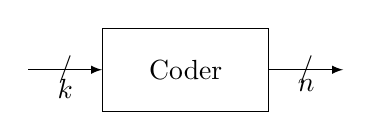
\begin{tikzpicture}[
                    node distance=2cm,
                    >=latex
                    ]

                    \node [coordinate] (input) {};
                    \node [draw, rectangle,right of = input, minimum height=3em, minimum width=6em] (block) {Coder};
                    \node [coordinate, right of = block] (output) {};
                    
                    \draw[draw,->] (input) -- node[midway]{$/$} node[below]{$k$} (block);
                    \draw[->] (block) -- node[midway]{$/$} node[below]{$n$} (output);
                \end{tikzpicture}    
            \label{Def codice forma sistematica}
            \end{figure}
            \begin{figure}[H]
                \centering 
                \includegraphics[width = 8cm]{media/forma sistematica.png}
            \label{matrice forma sistematica}
            \end{figure}
            \paragraph{Esempio Codice a ripetizione:}
            $R = \frac{1}{3},\ k=1,\ n=3$
            \begin{table}[H]
                \centering
                \begin{tabular}{|c|c|}
                \hline
                Bit i  ingresso & Parola codificata \\ \hline
                0               & {[}000{]}         \\ \hline
                1               & {[}111{]}         \\ \hline
                \end{tabular}
            \end{table}
            La matrice generatirce del codice é $G = [111]$, e la distanza minima $d_{min} = 3$\\

            \paragraph{Esempio Codice a controllo di paritá:}
            $R = \frac{7}{8},\ k=7,\ n=8$, ogni 7 bit ne aggiunge uno di controllo di paritá, 1 se il numero di "1" é diapari,
            0 se il numero di "1" é diapari.


            \noindent La matrice generatirce del codice:
            \[
                G = [I_7,1_7]
            \]
            \noindent La distanza minima é $d_{min} = 2$, se cambio uno dei 7 bit della parola
            cambio automaticamente il bit di paritá, quindi cambiare 1 bit in realtá ne cambia 2.\\

            \noindent Il prodotto $u\dotproduct 1_7 = \sum_{i=1}^{7}u_i$, puó essere scritto come una soma modulo 2, vale 0 se il numero di 
            occorrenze di "1" é pari e 1 altrimenti. Non facciamo altro che calcolare il bit di paritá della parola $u$.
            
            \paragraph{Definizione:} Due codici lineari $\mathcal{C}_1(k,n)$ e $\mathcal{C}_2(k,n)$ in $GF(2)$ sono equivalenti se uno é ottenuto dall'altro
            attraverso una permutazione delle posizioni del codice.

            \paragraph{Teorema:} Due matrici generatrici $G_1$ e $G_1$ in $GF(2)$ generano due codici equivalenti se una puó essere ottenuta dall'altra
            da una sequenza di operazioni come:
            \begin{itemize}
                \item Permutazione delle righe.
                \item Combinazione lineare delle righe.
                \item Permutazione delle colonne.
            \end{itemize}
            
            \paragraph{Teorema:} Qualsiasi codice lineare a blocchi é equivalente ad un codice in forma sistematica.

            \paragraph{Propietá degli spazi:}
            \begin{itemize}
                \item {
                    Dato il sottospazio $\mathcal{C} \subset \mathcal{V}_n$ di dimensione $k$, esiste un sottospazio ortogonale (null space)
                    $\mathcal{C}^\perp \subset \mathcal{V}_n$ di dimensione $n-k$ definito da una matrice $H\in (n-k) \times n$:
                    \[
                        GH^T = 0_{n-k}  
                    \]
                }
                \item {
                    La base di $\mathcal{C}^\perp$ é costituita dalle $n-k$ righe della matrice $H$, per cui ogni elemento $t\in \mathcal{C}^\perp$ puó 
                    essere rappresentato:
                    \[
                        t = vH = \sum_{i=1}^{n-k}v_ih_i  
                    \]
                }
                \item {
                    Per ogni $x\in \mathcal{C}$ e per ogni $t\in \mathcal{C}^\perp$ si ha:
                    \[
                        xt^T = uGH^Tv^T = 0
                    \]  
                }
            \end{itemize}
        \subsubsection{Matrice di controllo di paritá}\label{Matrice di controllo di parita}\index{Matrice di controllo di paritá}
            La matrice $H$ é la matrice di controllo di paritá del codice. Per costruzione $\forall x \in \mathcal{C}$ vale:
            \begin{gather}
                    xH^T = uGH^T = 0 \nonumber \\
                    H\in (n-k) \times n\nonumber 
            \end{gather}
            La matrice $H$ non é unica, ma se il codice é sistematico posso ricavarla in un'altra forma:
            \begin{gather}
                H = [P^T,I_{n-k}] = 0 \nonumber \\
                H\in (n-k) \times n,\ I\in (n-k)\times (n-k),\ P^T\in (n-k) \times k \nonumber
            \end{gather}
            Se fosse $\neq 0$ ció che é stato ricevuto non é una parola di codice.
            
            \paragraph{Esempio codice a ripetizione e controllo di paritá:}
                $R = \frac{1}{3},\ k=1,\ n=3,\ n-k=2$ ho la matrice a controllo di paritá:
                \[
                    H= [P^T,I_2] =
                        \begin{bmatrix}
                        1 & 1 & 0\\
                        1 & 0 & 1
                        \end{bmatrix}  
                \]  
                Per un codice con $R = \frac{7}{8},\ k=7,\ n=8,\ n-k=1$ la matrice a controllo di paritá:
                \[
                    H= [P^T,I_1] = 1_8^T
                \]
        \subsubsection{Propietá dei codici a blocco}
            \paragraph{Teorema:} La distanza minima del codice a blocco $\mathcal{C}(k,n)$ si puó calcolare come il 
            peso di Hamming minimo tra tutte le parole di codice:
            \begin{align}
                d_{min}(\mathcal{C}) &= \underset{x_i,x_j\in\mathcal{C}}{\min} d_H(x_i,x_j) = \underset{x_i,x_j\in\mathcal{C}}{\min} d_H(x_i+x_j,x_j+x_j)\nonumber \\
                                     &= \underset{x_i,x_j\in\mathcal{C}}{\min} d_H(x_i+x_j,0_{1,n}) \overset{[x_i+x_j\in\mathcal{C}]}{\Rightarrow} \underset{x_i\in\mathcal{C}}{\min}\ w(x_i)\nonumber
            \end{align}
            \paragraph{Capacitá di rivelare errori (Error Detection):}
                Su un canale $BSC$ senza memoria (\ref{BSC system moretti}), la $n-upla\ y$ a valle del decisore puó essere rappresentata:
                \[
                    y=x+e  
                \] 
                Dove $e$ é il vettore di errori introdotto dal canale, se il canale non introduce errori: $e = 0_{1,n}$
                Sia $x$ la parola di codice trasmessa e $y=x+e$ la corrispondente sequenza di $n$ bit ricevuta. supponiamo che il canale 
                introduca un numero di errori:$w(e) > 0$, si dice:
                \begin{itemize}
                    \item {
                        Errore Rivelabile\index{Errore Rivelabile}: se $y$ non é una parola di codice, $y\notin\mathcal{C}(k,n) $
                    }
                    \item {
                        Errore Non Rivelabile\index{Errore Non Rivelabile}: se $y$ é una parola di codice ma non quella trasmessa, $w(e) \geq d_{min}$ 
                    }
                \end{itemize} 
                \subparagraph{Teorema:} Il codice $\mathcal{C}(k,n)$ é in grado di rivelare con certezza fino a $d_{min}-1$ errori.
                \begin{itemize}
                    \item {
                        Se $d(x,y)<d_{min}$: $y$ non puó essere una parola di codice, altrimenti vorrebbe dire cge esistono due parole di codice la cui distanza 
                        é minore di $d_{min}$.
                    }
                    \item {
                        Se $d(x,y)=d_{min}$: esiste almeno una parola di codice $c\in\mathcal{C}(k,n),\ c \neq x$ tale che $d(x,c)=d_{min}$, se $y=c$ l'errore non 
                        puó essere rivelato. 
                    }
                \end{itemize}
            \paragraph{Strategia di decodifica a massima verosomiglianza:}
                Sia $y$ il vettore ricevuto a seguito della trasmissione su $BSC$ , la strategia di decodifica a massima verosomiglianza (ML, maximum likelihood) 
                consiste nel trovare il vettore $\hat{x}$ che, tra tutte le $2^k$ possibili parole di codice $x$, massimizza la probabilitá condizionata 
                $P(y|x)$:
                \[
                    \hat{x} = \arg \underset{x\in\mathcal{C}}{\max}\ P(y|x)
                \]
                Poiché gli eventi di errore sono indipendenti da bit a bit, posso riscrivere la probabilitá condizionata come il prodotto delle probabilitá condizionate
                ottenute per ciascun bit trasmesso:
                \[
                    P(y|x) = \prod_{\ell=1}^{n} P(y_\ell|x_\ell)
                \]
                Lavorando in $GF(2)$ la probabilitá $P(y_\ell|x_\ell)$ puó assumere solo 2 valori:
                \[
                    P(y_\ell|x_\ell) = 
                    \begin{cases}
                        1-p &se\ P(y_\ell =x_\ell|x_\ell)\nonumber \\    
                        p   &se\ P(y_\ell \neq x_\ell|x_\ell)\nonumber     
                    \end{cases}
                \] 
                Osservazione: La distanza di Hamming $d_H(x,y)$ misura il numero di posizione diverse tra $x$ e $y$, quindi $n-d_H(x,y)$ minura il numero di posizioni
                uguali tra $x$ e $y$.

                La probabilitá $P(y|x)$ si calcola:
                \[
                    P(y|x) = p^{d_H(x,y)}(1-p)^{n-d_H(x,y)} =(1-p)^{n}\left(\frac{p}{1-p}\right)^{d_H(x,y)} 
                \]
                Mi interessa scegliere un $x$ che massimizza $\left(\frac{p}{1-p}\right)^{d_H(x,y)}$, é un valore $<1$:
                \begin{itemize}
                    \item {
                        RICONtROLLA LEIZONE
                        Se ho la $d_H(x,y)$ piccola ho la probabilitá minore di errore.
                    }
                    \item {
                        Se ho la $d_H(x,y)$ alta ho la probabilitá di errore alta.
                    }
                \end{itemize}
                
            \paragraph{Decisione a massima verosomiglianza:}\label{Decisione a massima verosomiglianza}\index{Decisione a massima verosomiglianza}
                La parola di codice decisa $\hat{x}$ é quella che minimizza la distanza dalla parola $y$ ricevuta:
                \[
                    \hat{x} = \arg \underset{x\in\mathcal{C}}{\max}\ P(y|x) = \arg \underset{x\in\mathcal{C}}{\min}\ d_H(y,x)
                \]
                Scelgo $x$ tale che mi dia la minima distanza ma RICONtROLLA LEIZONE
                \subparagraph{Ricevitore ML ottimo:}\index{Ricevitore ML ottimo} Il ricevitore ML ottimo é il ricevitore a distanza minima, il ricevitore
                che associa alla sequenza di $n$ bit ricevuta $y$, la parola di codice $x$ che minimizza la $d_H(y,x)$.
                \subparagraph{Ricevitore ML error correction:}\index{Ricevitore ML error correction} Il ricevitore ML é in grado di correggere cn successo tutti quegli errori
                $e$ per cui la parola ricevuta $y = x+e$ é comunque piú vicina alla parola trasmessa $x$ che a qualsiasi altra parola del codice.
                
                Per ogni vettore $v\in\mathcal{V}_n$ e un reggio $r$ esiste una "sfera" di raggio $r$ i cui elementi sono tutti quei vettori in $\mathcal{V}_n$ che hanno
                distanza di Hamming da $v$ minore o uguale a $r$

                \begin{figure}[H]
                    \centering 
                    \includegraphics[width = 4cm]{media/sfera di amming.png}
                \label{sfera di Hamming}
                \end{figure}
                Se adottiamo un ricevitore ML, il numero massimo di errori che il codice $\mathcal{C}(k,n)$ é in grado di correggere é il massimo raggio $t$ per cui le sfere centrate nelle 
                parole di codice di $\mathcal{C}(k,n)$ sono tutte tra loro disgiunte.
            \paragraph{Capacitá di correggere errori (Error Correction):}
                \subparagraph{Teorema:}\begin{sloppypar}
                   Un codice lineare a blocco puó correggere fino a ${t_{max} = \left\lfloor \frac{d_{min}-1}{2} \right\rfloor}$ errori: $2t_{max}+1 \leq d_{min} \leq 2t_{max}+2$.
                \end{sloppypar}
                    
                \begin{sloppypar}
                    La condizione per cui le sfere di raggio $t$ che circondano le parole di codice siano disgiunte é che ${2t_{max} < d_{min}\Rightarrow t_{max} < \frac{d_min}{2}}$.
                    Altrimenti se fosse  ${2t_{max} \geq d_{min}}$ ci sarebbero almeno die parole $x_1$ e $x_2$ la cui distanza ${d_H(x_1,x_2) = d_{min} < 2t_{max} }$ e le que sfere di raggio
                    $t$ avrebbero almno un unto in comune.
                \end{sloppypar}
                
                \begin{sloppypar}
                    Consideriamo il codice $\mathcal{C}(k,n)$ che ha una certa $d_{min}$ e $t_{max}$ tale che ${2t_{max}+1 \leq d_{min}}$. Sia $x\in\mathcal{C}(k,n)$ la parola trasmessa,
                    ${y = x+e}$ la corrispondente sequenza di $n$ bit ricevuta e $c\in\mathcal{C}(k,n)$ un'altra generica parola di codice. Grazie alla disuguaglianza triangolare ho:
                    \[
                        d_H(x,y) + d_H(c,y) \geq d_H(x,c) \Rightarrow d_H(c,y) \leq d_H(x,c) - d_H(x,y)  
                    \]
                    per ipotesi ho anche:
                    \[
                        d_H(x,c) \geq d_{min} \geq 2t_{max}+1 
                    \]
                    Supponiamo che il canale introduca un certo numero di errori ${t\leq} t_{max}$, cosí da avere $d_H(x,y) = t$:
                    \[
                        d_H(c,y) \geq 2t_{max}+1 -t > t_{max} \geq t = d_H(x,y)   
                    \]   
                \end{sloppypar}
                
    \subsection{Codici di Hamming}
        I codici di Hamming $\mathcal{C}_H(m)$ sono definiti a partire da un parametro: $m \geq 2$
        \[
            n = 2^m-1,\ k = 2^m-m-1 = n-m
        \]
        \subparagraph{Matrice di controllo di paritá:} per definizione la matrice $H \in (n-k)\times n$, ma per i codici di Hamming la matrice $H$ ha dimensione:
        $H \in m\times (2^m-1)$.

        \subparagraph{Matrice di paritá:} Per un codice di Hamming sistematico la matrice di parità $P\in k \times m$ viene costruita cosí che le colonne di $H = [P^T,I_{n-k}]$
        siano tutte le possibili $2^m-1$ combinazioni di $m$ bit (esclusa la $n-upla$ di tutti 0)

        \subsubsection{Il codice $\mathcal{C}_H(2)$}
            \begin{sloppypar}
                Il codice a ripetizione ${R=\frac{1}{3}}$ con ${m=2\Rightarrow n=3,\ k=1}$ ha come matrice di controllo di paritá $H$:
                \[
                    H = \begin{bmatrix}
                            1  & 1 & 0 \\
                            1  & 0 & 1 \\
                        \end{bmatrix} 
                \]
                Che é la matrice corrispondente a un codice di Hamming $\mathcal{C}_H(2)$, poiché rappresenta tutte le possibili combinazioni di 2 bit
            \end{sloppypar}

        \subsubsection{Il codice $\mathcal{C}_H(3)$}
        \begin{gather}
            m=3,\ n=7,\ k=4,\ R=\frac{4}{7} \nonumber \\
            H = \begin{bmatrix}
                1 & 0 & 1 & 0 & 1 & 0 & 1\\
                0 & 1 & 1 & 0 & 0 & 1 & 1\\
                0 & 0 & 0 & 1 & 1 & 1 & 1
            \end{bmatrix}  \nonumber
        \end{gather}
        Posso ricavare la matrice generatrice $G$ scrivendo la matrice $H$ come se l'avessi ottenuta da una matrice $G\in k \times n$ di un codice sistematico (\ref{Matrice di controllo di parita}):
        \[
            H = [P^T,I_{n-k}] =\begin{bmatrix}
                                 1  & 1 & 0 & 1 & | & 1  & 0 & 0\\
                                 1  & 0 & 1 & 1 & | & 0  & 1 & 0\\
                                 0  & 1 & 1 & 1 & | & 0  & 0 & 1
                            \end{bmatrix} 
        \]
        La cui matrice generatrice con $I \in k \times k$ é:
        \[
            G = [I_{k},P] =\begin{bmatrix}
                                 1  & 0 & 0 & 0 & | & 1  & 1 & 0\\
                                 0  & 1 & 0 & 0 & | & 1  & 0 & 1\\
                                 0  & 0 & 1 & 0 & | & 0  & 1 & 1\\
                                 0  & 0 & 0 & 1 & | & 1  & 1 & 1
                            \end{bmatrix} 
        \]
        Possiamo vedere come la matrice di paritá faccia conrolli su combinazioni diverse di bit in ingresso $p = uP$:
        \begin{gather}
            p_1 = u_1+u_2+u_4 \nonumber\\
            p_2 = u_1+u_3+u_4 \nonumber\\
            p_3 = u_2+u_3+u_4 \nonumber
        \end{gather}
        Il vettore di uscita dal codificatore sará quindi $x = uG = [u,p_1,p_2,p_3]$, tale matrice di paritá ci permette di aumentare la distanza di Hamming
        tra le parole
        \subparagraph{Distanza minima:} La distanza minima di un qualsiasi codice di Hamming $\mathcal{C}_H(m)$ é $d_{min}(\mathcal{C}_H(m)) = 3$.

        \noindent Dimostrazione: 
        \begin{enumerate}
            \item {
                $d_{min} = \underset{x\in\mathcal{C}}{\min}\ w(x)$  
            }
            \item {
                $x\in\mathcal{C}\ se\ xH^T= 0$ e le colonne di $H$ sono tutte le possibili combinazioni dei bit $m$ bit
            }
        \end{enumerate}
        Perché $3$ é il numero minimo di colonne che mi permette di ottenere $0$ ($2$), quindi $d_{min}(\mathcal{C}_H(m)) = 3$.
        
        %Ne consegue che aumentando il numero di bit trasmessi diminuisco la ridondanza, ma la mia distanza di Hamming rimane sempre la stessa.
    \subsection{Decodifica per codici a blocco}
        Dato il vettore ricevuto:
        \[
            y = x+e
        \]
        Il decisore ottimo selezione la parola di codice $\hat{x}$:
        \[
            \hat{x} = \arg \underset{x\in\mathcal{C}}{\max}\ P(y|x) = \arg \underset{x\in\mathcal{C}}{\min}\ d_H(y,x)   
        \]
        Per ottenere $\hat{x}$ é necessario fare $2^k$ confronti tra il vettore ricevuto $y$ e tutte le parole di codice $\mathcal{C}(k,n)$, 
        la complessitá cresce esponenzialmente con $k$.

        Un approccio alternativo é quello di osservare il vettore errore e la probabilitá condizionata:
        \begin{gather}
            y= x+e \Rightarrow x = y+e,\ e = y-x\nonumber\\
            P(x|y) = P(x+e|x) = P(e|y+e\in\mathcal{C})\nonumber
        \end{gather}
        Posso ottenera la stima di $x$ come:
        \[
            \hat{x} = \arg \underset{x\in\mathcal{C}}{\max}\ P(y|x) =y+ \arg \underset{e}{\max}\ P(e|y+e\in\mathcal{C})   
        \]
        Invece di stimare $\hat{x}$ si stima il vettore $\hat{e}$ piú probabile
        \begin{align}
            \hat{e} &= \arg \underset{e}{\max}\ P(e|y+e\in\mathcal{C}) = \arg \underset{e|y+e\in\mathcal{C}}{\max}\ p^{w(e)}(1-p)^{n-w(e)} \nonumber \\
                    &= \arg \underset{e|y+e\in\mathcal{C}}{\max}\ \left(\frac{1-p}{p}\right)^{-w(e)} = \arg \underset{e|y+e\in\mathcal{C}}{\min}\ w(e)  \nonumber 
        \end{align}
        La decodifica sceglie tra tutti i possibili vettori errore $e$ tali che $y+e\in\mathcal{C}$ quello che ha il peso di Hamming minimo, cioé il minimo numero di 
        errori (Massima Verosomiglianza). Una volta stimato $\hat{e}$:
        \[
            \hat{x} = y-\hat{e} = y+\hat{e} = x+(\hat{e}+e)=
            \begin{cases}
                x &se\ \hat{e} = e\nonumber\\    
                x_1\neq x &se\ \hat{e} \neq e\nonumber    
            \end{cases}     
        \]
        \subsubsection{Coset}
            Sia $\mathcal{C}(k,n)$ un codice a blocco e sia $v\in \mathcal{V}_n$ un vettore di $n$ cifre binarie, si definisce $coset$ di
            $\mathcal{C}(k,n)$ individuato da $v$ l'insieme:
            \[
                C_v = C+v=\{ x+v: x\in\mathcal{C} \}
            \]
        \subsubsection{Propietá dei coset}
            \begin{enumerate}
                \item {Qualsiasi vettore in $\mathcal{V}_n$ appartiene a un coset di $\mathcal{C}(k,n)$}
                \item {Ciascun coset contiene $2^k$ elementi}
                \item {Due coset o sono coincidenti o hanno intersezione nulla}
                \item {Ci sono $2^{n-k}$ coset distinti}
                \item {Se $v_1$ e $v_2$ appartengono all ostesso coset, $v_1 + v_2 \in \mathcal{C}(k,n)$ é una parola di codice}
            \end{enumerate}
            \paragraph{Esempio di coset:}
                \begin{sloppypar}
                    Sia ${\mathcal{C}(2,3) = \{000,101,010,111\}}$. I coset di ${\mathcal{C}(2,3)}$: 
                \end{sloppypar}
                \begin{align}
                    \mathcal{C} + 000 = \{000,101,010,111\} = \mathcal{C}_0 \\
                    \mathcal{C} + 001 = \{001,100,011,110\} = \mathcal{C}_1 \\
                    \mathcal{C} + 010 = \{010,111,000,101\} = \mathcal{C}_0 \\
                    \mathcal{C} + 011 = \{011,110,001,100\} = \mathcal{C}_1 \\
                    \mathcal{C} + 100 = \{100,001,110,011\} = \mathcal{C}_1 \\
                    \mathcal{C} + 101 = \{101,000,111,010\} = \mathcal{C}_0 \\
                    \mathcal{C} + 110 = \{110,011,100,001\} = \mathcal{C}_1 \\
                    \mathcal{C} + 111 = \{111,010,101,000\} = \mathcal{C}_0 
                \end{align}
                Il numero di coset é $2^{n-k} = 2^{3-2} =2$.

            Si possono applicare i coset per la decodifica: $y=x+e$ dalla definizione di coset discende che i vettori $e$ e $y$
            appartengono allo stesso coset $\mathcal{C}_y$ e che i coset $\mathcal{C}_e$ e $\mathcal{C}_x$ sono coincidenti. Grazie alla propietá
            dei coset la somma di qualsiasi elemento di $\mathcal{C}_y$ con $y$ individua una parola di codice. Il vettore $e$ va scelto fre gli elementi
            di $\mathcal{C}_y$, la regola di decisione diveta:
            \[
                \hat{e} = \arg \underset{e}{\max}\ P(e|y+e\in\mathcal{C}) = \arg \underset{e\in\mathcal{C}_y }{\max}\ P(e) =\arg \underset{v\in\mathcal{C}_y }{\max}\ w(v)
            \] 
            Tra tutti i $2^k$ possibili vettori di $\mathcal{C}_y$, il principio di massima verosomiglianza dice che devo scegliere quello di peso minimo.
        \subsubsection{Algoritmo di decodifica}
            \begin{enumerate}
                \item Avendo ricevuto il vettore $y$ si trova un coset di appartenenza $\mathcal{C}_y$.
                \item {Si identifica il coset leader, la parola di peso minimo del coset $\mathcal{C}_y$, che é anche la parola di peso minimo del 
                coset di $\mathcal{C}_e$.}
                \item Il coset leader é la stima del vettore di errore $\hat{e}$
            \end{enumerate}
            \paragraph{Esempio di decodifica utilizzando i coset:}
                    Sia ${\mathcal{C}(2,4) = \{0000,1011,0101,1110\}}$ con $d_{min} = 2$, ho i coset: 
                \begin{align}
                    \mathcal{C} + 0000 = \{0000,1011,0101,1110\} \\
                    \mathcal{C} + 0001 = \{0001,1010,0100,1111\} \\
                    \mathcal{C} + 0010 = \{0010,1001,0111,1100\} \\
                    \mathcal{C} + 1000 = \{1000,0011,1101,0110\} 
                \end{align}
                Il numero di coset é $2^{n-k} = 2^{4-2} =4$. Il coset (2) non so quale coset leader scegliere hanno lo stesso peso di Hamming, ci
                troviamo in questo poiché la $d_{min}$ é molto bassa e ho il $50\%$ di possibilitá di sbagliare se il codice ricevuto capita in questo coset.
                Decodifichiamo:
                \begin{itemize}
                    \item {$y=[1101]\Rightarrow y\in (4),\text{coset leader:} [1000]\ \hat{x}=y+1000=0101$}
                    \item {$y=[1111]\Rightarrow y\in (2),\text{coset leader:} [0001] \vee [0100] \ \hat{x}=y+0001=1110$}
                \end{itemize}
        \subsubsection{Decodifica mediante sindrome}
            Si definisce sindrome di $y$ il vettore $s$ ottenuto dal prodotto di $y$ con la matrice di controllo di paritá:
            \[
                s = yH^T = (x+e)H^T = xH^T+eH^T = eH^T    
            \]
            \paragraph{Propietá:}
                \begin{itemize}
                    \item {
                        Tutti i membri di uno stesso coset hanno la stessa sindrome
                    }
                    \item {
                        $s \in 1 \times (n-k)$
                    }
                    \item {
                        Le $2^{n-k}$ sindromi sono associate ai $2^n-k$ diversi coset del codice $\mathcal{C}(k,n)$
                    }
                    \item {
                        Ciascuna sindrome é associata ai $2^k$ pattern di errore apparteenti allo stesso coset.
                    }
                \end{itemize}
            \paragraph{Procedura di decodifica:}
                \begin{enumerate}
                    \item {Calcola la sindrome $s = yH^T$}
                    \item {Associa la sindrome al coset leader corrispondente $s\rightarrow e_{CL}(s)$}
                    \item {Corregge l'errore sommando il coset leader alla $n-upla\ y$}
                \end{enumerate}
                La parola $\hat{x}$ é una parola di codice:
                \[
                    \hat{x}H^T= (y+e_{CL}(s))H^T = s+s =0   
                \]
                e per costruzione la parola di codice $\hat{x}$ minimizza la distanza di Hamming da $y$
        \subsubsection{Decodifica a sindrome: Codici di Hamming $m=3$}
            \begin{sloppypar}
                Il codice ha $d_{min} = 3$ ed é in grado di correggere esattamente un errore: ${t_{max} = \left\lfloor \frac{d_{min}-1}{2}\right\rfloor = 1}$. Si sceglie la matrice $H$
                in maniera che la tabella di decodifica associ alla sindrome il pattern di errore a peso 1 in cui il bit
                messo a 1 sia nella posizione corrispondente alla conversione della sindrome in decimale.
            \end{sloppypar}
            \begin{table}[H]
                \subfloat[Codice non sistematico]{
                    \begin{tabular}{cc}
                        \hline
                        Sindrome  & Coset Leader  \\ \hline
                        {[}000{]} & {[}0000000{]} \\
                        {[}100{]} & {[}1000000{]} \\
                        {[}010{]} & {[}0100000{]} \\
                        {[}110{]} & {[}0010000{]} \\
                        {[}001{]} & {[}0001000{]} \\
                        {[}101{]} & {[}0000100{]} \\
                        {[}011{]} & {[}0000010{]} \\
                        {[}111{]} & {[}0000001{]} \\ \hline
                        \end{tabular}
                }
                \hfill
                \subfloat[Codice sistematico]{
                    \begin{tabular}{cc}
                        \hline
                        Sindrome  & Coset Leader  \\ \hline
                        {[}000{]} & {[}0000000{]} \\
                        {[}100{]} & {[}0000100{]} \\
                        {[}010{]} & {[}0000010{]} \\
                        {[}110{]} & {[}1000000{]} \\
                        {[}001{]} & {[}0000001{]} \\
                        {[}101{]} & {[}0100000{]} \\
                        {[}011{]} & {[}0010000{]} \\
                        {[}111{]} & {[}0001000{]} \\ \hline
                    \end{tabular}
                }
            \end{table}
        \subsubsection{Esempio di decodifica}
            Un codice lineare a blocchi ha la seguente matrice di controllo di parità:
            \[
                H=
                    \begin{bmatrix}
                    1 & 0 & 1 & 1 & 0 & 0\\
                    1 & 1 & 0 & 0 & 1 & 0\\
                    0 & 1 & 1 & 0 & 0 & 1
                    \end{bmatrix}  
            \]  
            \begin{enumerate}
                \item {Determinare la matrice generatrice:
                
                }
                \item {Decodificare la parola $y = [110110]$ ed identificare la parola di codice trasmessa:
                
                }
            \end{enumerate}



































